\subsection{Ausführung}
Für die Ausführung und Verwendung der Simulink Modelle sollte vorzugsweise die PSP Anleitung konsultiert werden. Auf mehreren Seiten ist der Vorgang sowie Projekteinstellungen detailliert und ausführlich erklärt.\\
Anbei wird eine Flugregelung erzeugt, welche auf dem Pixhawk läuft und über das Simulink gesteuert werden kann. Das Vorgehen basiert auf den folgenden Schritten:\\

\noindent
\textbf{Modellentwurf}\\
Das Modell in Abbildung \ref{fig:psp_modell} enthält den Flugregler, welcher später auf dem Pixhawk laufen soll. Der Regler berechnet anhand den Sensordaten die Stellgrössen der Aktuatoren.
\begin{figure}[H]
  \begin{center}
  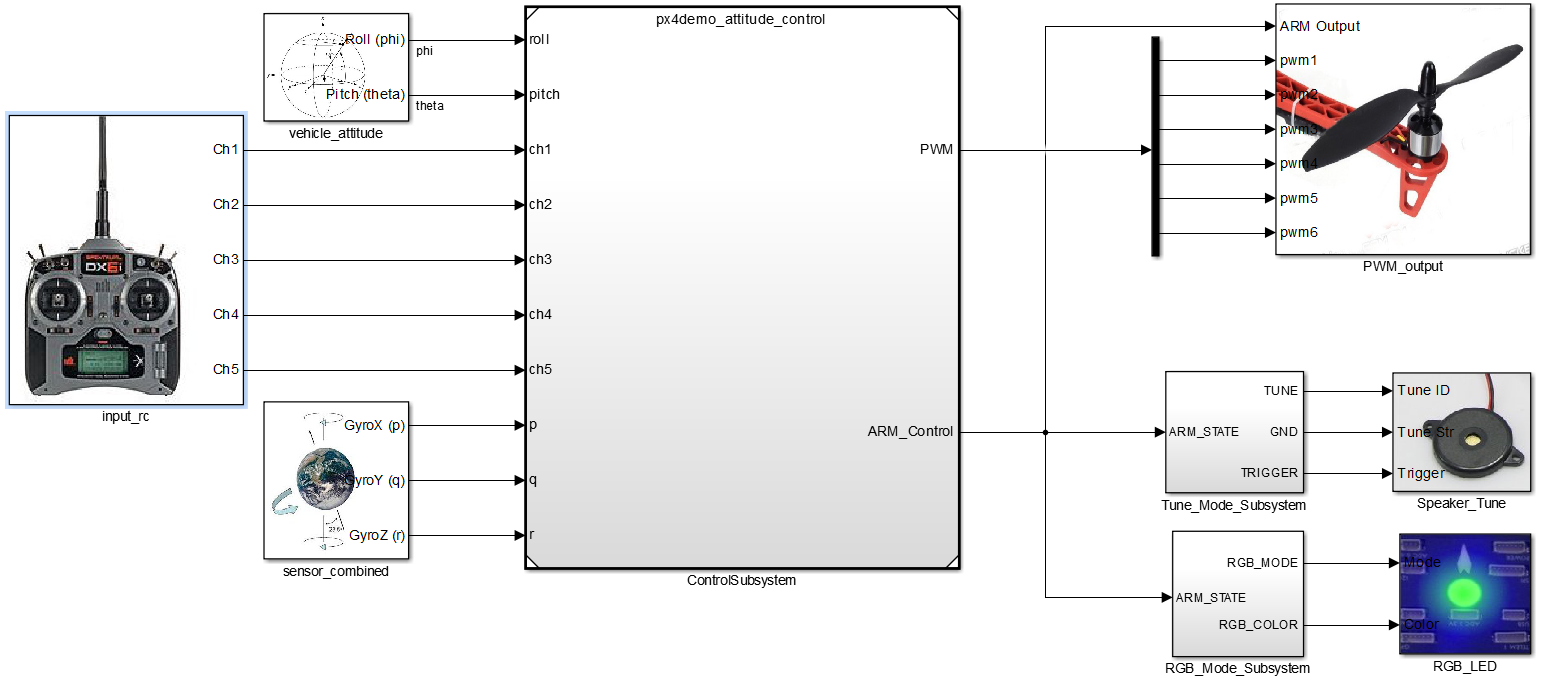
\includegraphics[scale=0.3]{pic/40_psp/psp_model.png}
  \caption{Simulink Modell}
  \label{fig:psp_modell}
  \end{center}
\end{figure}

\noindent
\textbf{Projekteinstellungen}\\
Eine Vielzahl von Einstellungen muss für den Code Composer vorgenommen werden. Je nach Verwendungszweck weichen diese ab.

\begin{figure}[H]
  \begin{center}
  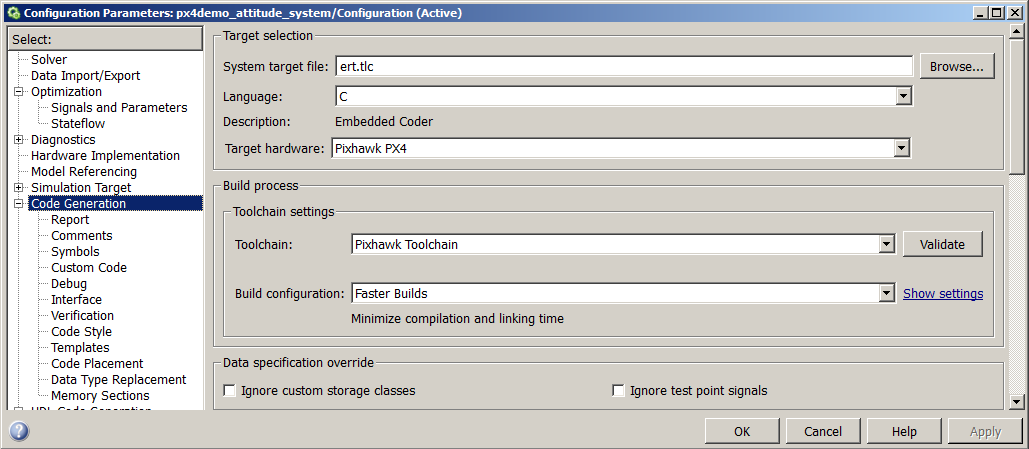
\includegraphics[scale=0.3]{pic/40_psp/psp_settings.png}
  \caption{Projekteinstellungen}
  \label{fig:psp_config}
  \end{center}
\end{figure}

\noindent
\textbf{Codegeneration}\\
Durch bestätigen des Knopfs in Abbildung \ref{fig:psp_generate} wird aus dem Simulink Blockschaltbild lauffähigen C Code generiert. Dieser Programmcode enthält mehrere Apps, welche automatisch auf das Pixhawk geladen werden. In Abbildung \ref{fig:psp_diagnostic} ist der Simulink Diagnostic Viewer ersichtlich. Hier wird aufgezeigt, dass der C Code erfolgreich zu einer .elf Datei kompiliert wurde und auf das Pixhawk geladen würde.

\begin{figure}[H]
  \begin{center}
  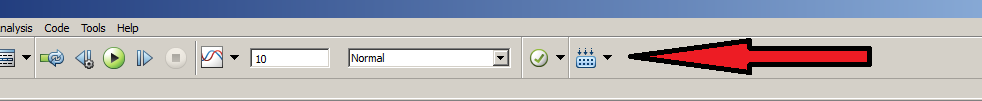
\includegraphics[scale=0.3]{pic/40_psp/psp_generate.png}
  \caption{Code generieren und hochladen}
  \label{fig:psp_generate}
  \end{center}
\end{figure}

\begin{figure}[H]
  \begin{center}
  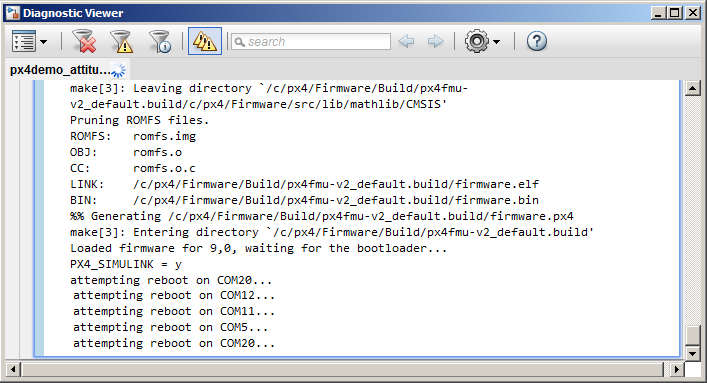
\includegraphics[scale=0.3]{pic/40_psp/psp_upload.png}
  \caption{Diagnostic Viewer}
  \label{fig:psp_diagnostic}
  \end{center}
\end{figure}


\noindent
\textbf{Simulation / realer Test}\\
Der Flugregler aus Abbildung \ref{fig:psp_modell} ist nun auf dem Pixhawk implementiert. Das Modell kann auf zwei Arten gestartet werden:
\begin{itemize}
\item Durch den 'run' Knopf im Simulink
\item Mit dem nsh Kommando px4\_simulink\_app start
\end{itemize}

\medskip

